% !TEX root = ../main.tex

\begin{frame}{Closeup Shot}
	\begin{itemize}
		\item Show the head and upper part of the body
		\item Leave the width of one hand above the head
		\item Eyes should be close to the upper third line
	\end{itemize}
\end{frame}

\begin{frame}{Closeup Shot: Good Example}
	\begin{figure}
		\centering
		\includegraphics[width=0.75\textwidth]{images/closeup1.jpg}
		\caption{Good closeup shot}
	\end{figure}
\end{frame}

% TODO: Replace with a screenshot from voctomix 2
\begin{frame}{Closeup Shot: Good Example}
	\begin{figure}
		\centering
		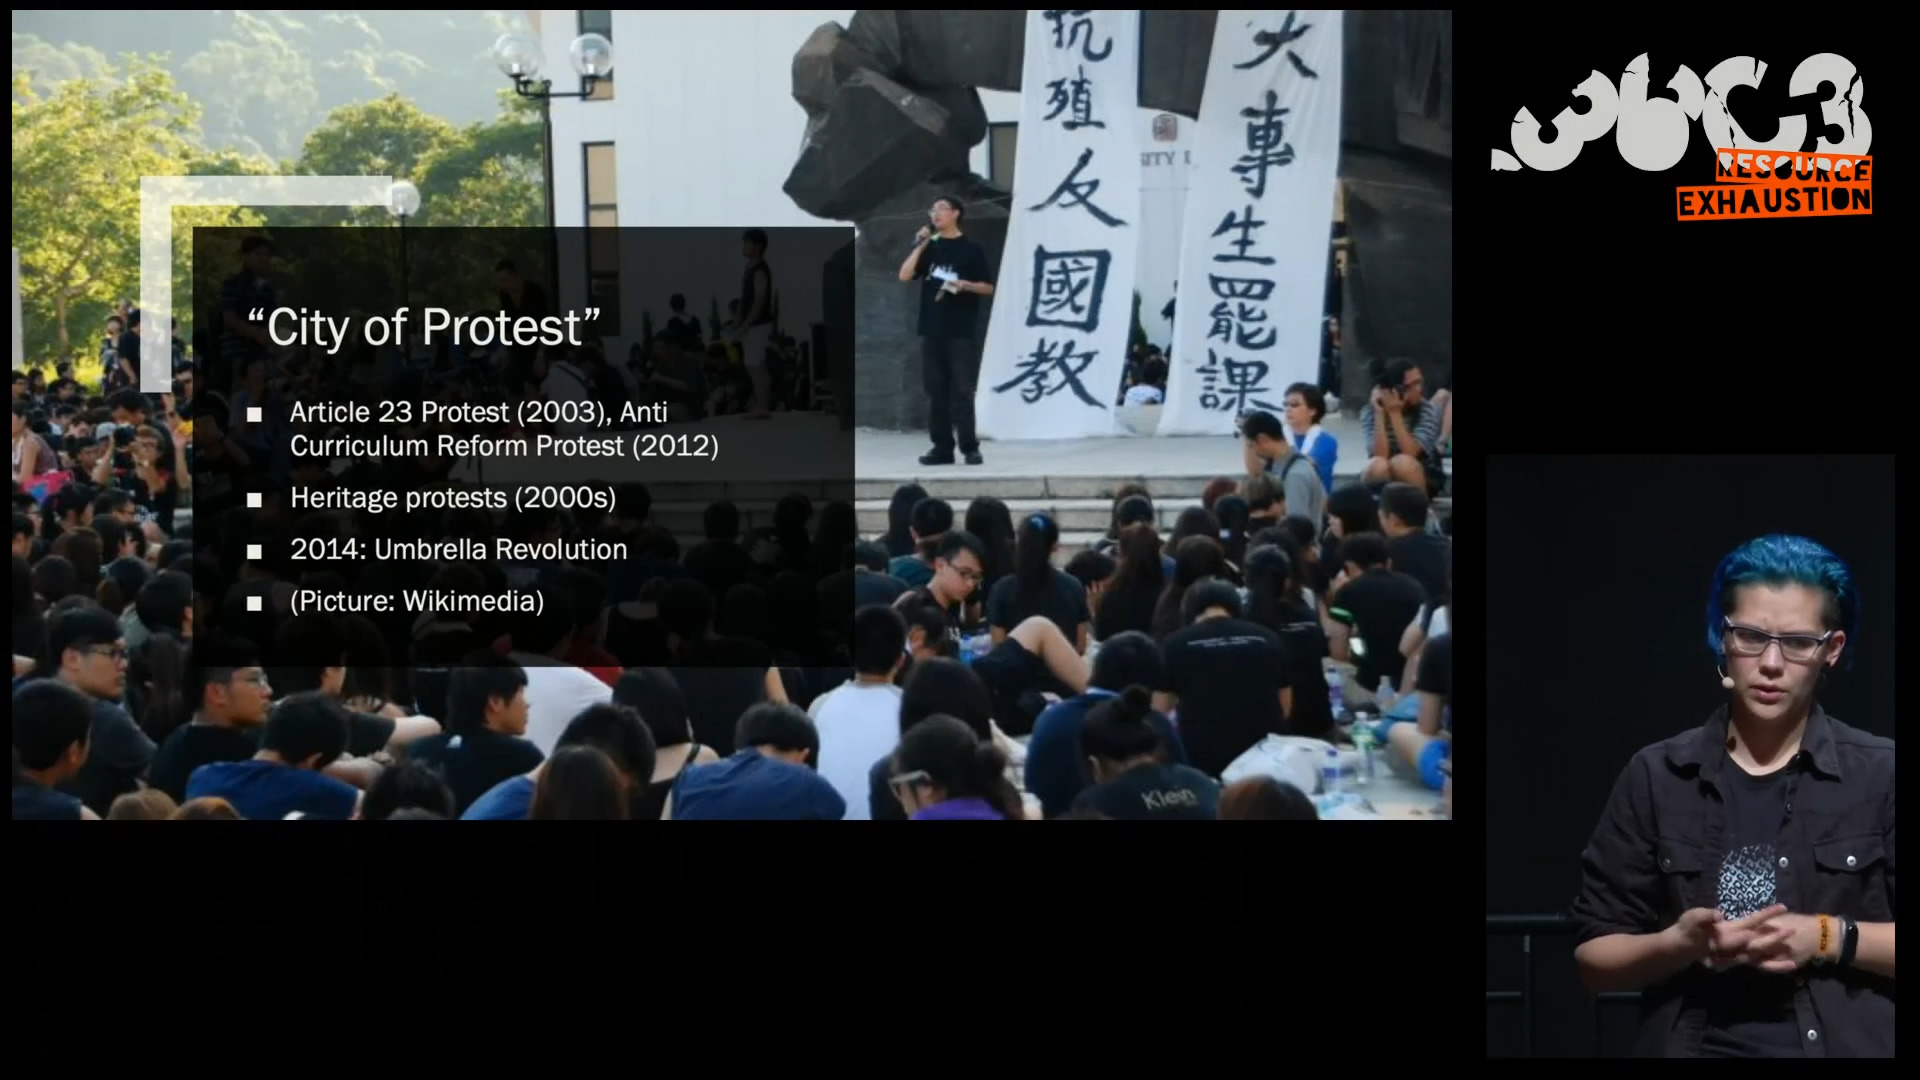
\includegraphics[width=0.75\textwidth]{images/closeup2.jpg}
		\caption{Good closeup in Lecture Mode}
	\end{figure}
\end{frame}

\begin{frame}{Closeup Shot: Bad Example}
	\begin{figure}
		\centering
		\includegraphics[width=0.75\textwidth]{images/closeup-bad1.png}
		\caption{Half a head - not good}
	\end{figure}
\end{frame}

\begin{frame}{Closeup Shot: Bad Example}
	\begin{figure}
		\centering
		\includegraphics[width=0.75\textwidth]{images/closeup-bad2.png}
		\caption{Too far out for a good Lecture Mode image}
	\end{figure}
\end{frame}

\begin{frame}{Medium Shot: Good 1}
	\begin{figure}
		\centering
		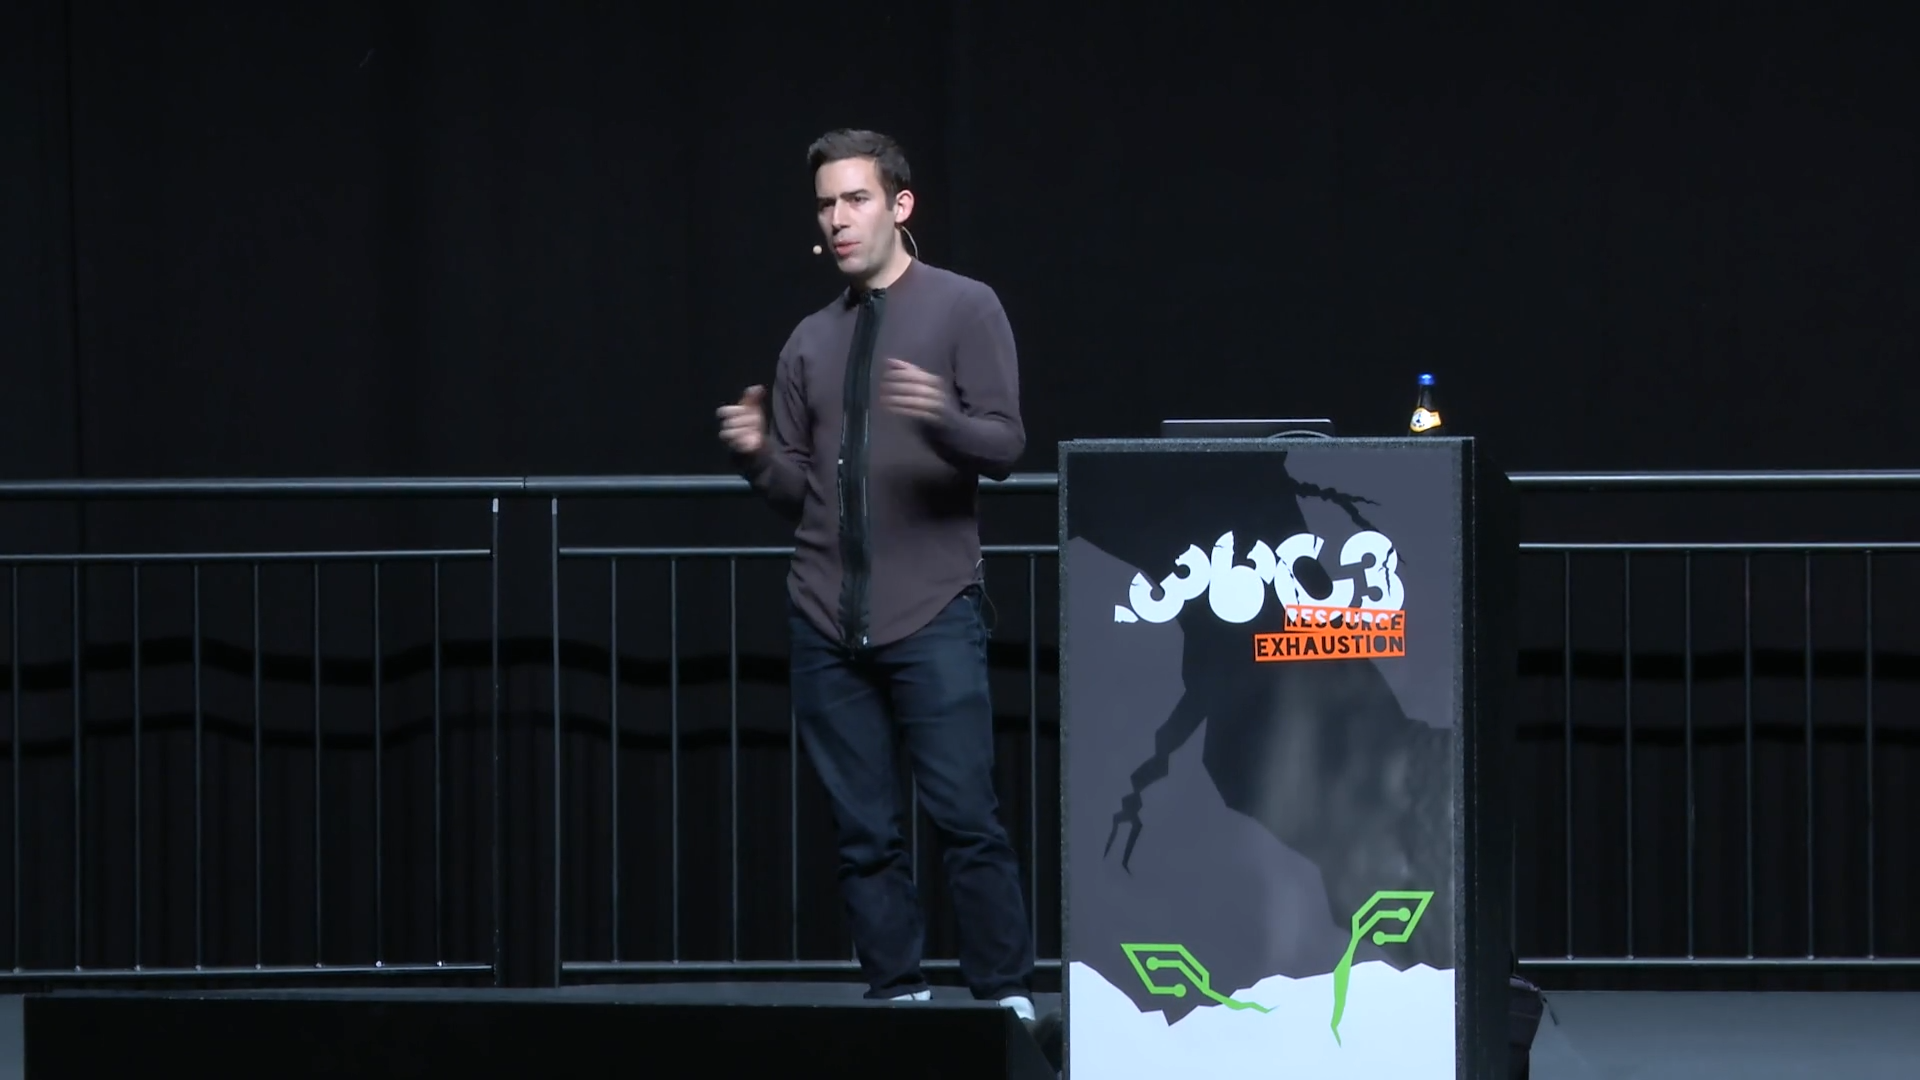
\includegraphics[width=0.75\textwidth]{images/medium1.png}
		\caption{One person, the lectern and some context}
	\end{figure}
\end{frame}

\begin{frame}{Medium Shot: Good 2}
	\begin{figure}
		\centering
		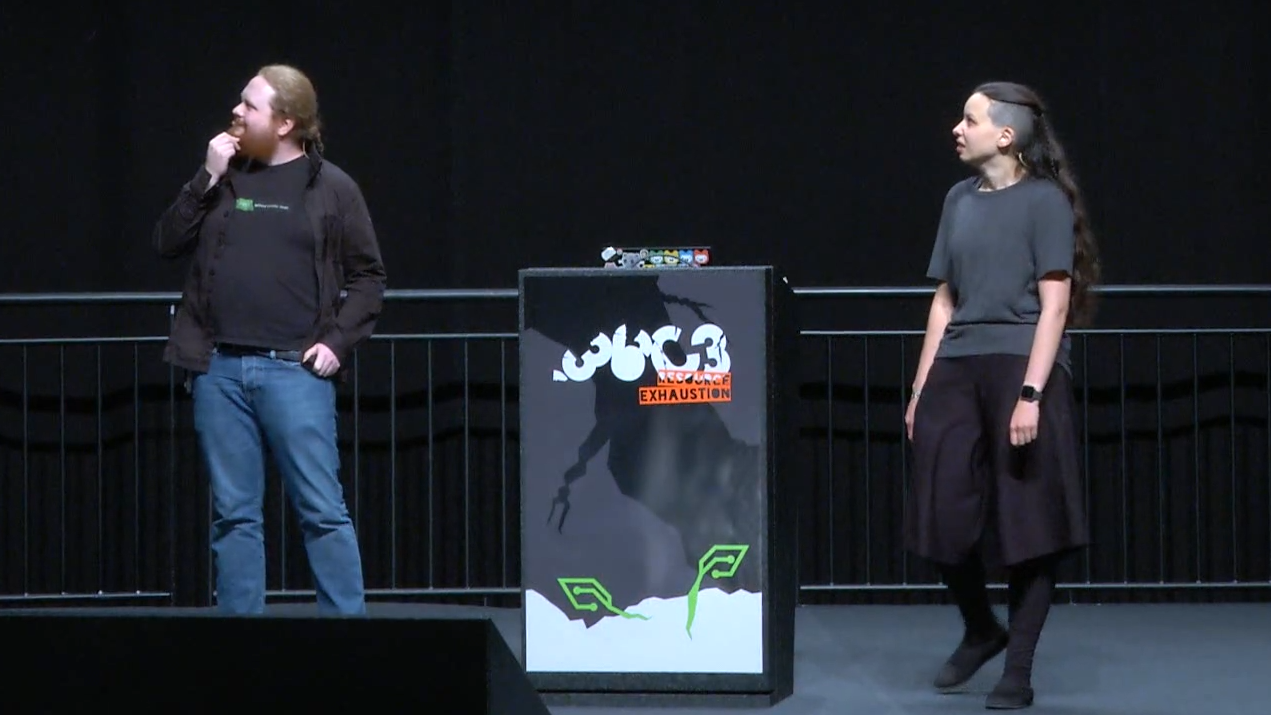
\includegraphics[width=0.75\textwidth]{images/medium2.png}
		\caption{Two persons on stage}
	\end{figure}
\end{frame}

\begin{frame}{Overview}
	\begin{itemize}
		\item Shows the complete stage and the people on it
		\item Heads of the crowd are OK, if it's dark enough
		\item Don't use this camera to show the slides - use lecture mode instead
		\item Locked off, do not move.
	\end{itemize}
\end{frame}

\begin{frame}{Wide Shot: Good Example}
	\begin{figure}
		\centering
		\includegraphics[width=0.75\textwidth]{images/wide-shot.jpeg}
	\end{figure}
\end{frame}
